\documentclass[serif]{beamer}\usepackage[]{graphicx}\usepackage[]{color}
%% maxwidth is the original width if it is less than linewidth
%% otherwise use linewidth (to make sure the graphics do not exceed the margin)
\makeatletter
\def\maxwidth{ %
  \ifdim\Gin@nat@width>\linewidth
    \linewidth
  \else
    \Gin@nat@width
  \fi
}
\makeatother

\definecolor{fgcolor}{rgb}{0.345, 0.345, 0.345}
\newcommand{\hlnum}[1]{\textcolor[rgb]{0.686,0.059,0.569}{#1}}%
\newcommand{\hlstr}[1]{\textcolor[rgb]{0.192,0.494,0.8}{#1}}%
\newcommand{\hlcom}[1]{\textcolor[rgb]{0.678,0.584,0.686}{\textit{#1}}}%
\newcommand{\hlopt}[1]{\textcolor[rgb]{0,0,0}{#1}}%
\newcommand{\hlstd}[1]{\textcolor[rgb]{0.345,0.345,0.345}{#1}}%
\newcommand{\hlkwa}[1]{\textcolor[rgb]{0.161,0.373,0.58}{\textbf{#1}}}%
\newcommand{\hlkwb}[1]{\textcolor[rgb]{0.69,0.353,0.396}{#1}}%
\newcommand{\hlkwc}[1]{\textcolor[rgb]{0.333,0.667,0.333}{#1}}%
\newcommand{\hlkwd}[1]{\textcolor[rgb]{0.737,0.353,0.396}{\textbf{#1}}}%

\usepackage{framed}
\makeatletter
\newenvironment{kframe}{%
 \def\at@end@of@kframe{}%
 \ifinner\ifhmode%
  \def\at@end@of@kframe{\end{minipage}}%
  \begin{minipage}{\columnwidth}%
 \fi\fi%
 \def\FrameCommand##1{\hskip\@totalleftmargin \hskip-\fboxsep
 \colorbox{shadecolor}{##1}\hskip-\fboxsep
     % There is no \\@totalrightmargin, so:
     \hskip-\linewidth \hskip-\@totalleftmargin \hskip\columnwidth}%
 \MakeFramed {\advance\hsize-\width
   \@totalleftmargin\z@ \linewidth\hsize
   \@setminipage}}%
 {\par\unskip\endMakeFramed%
 \at@end@of@kframe}
\makeatother

\definecolor{shadecolor}{rgb}{.97, .97, .97}
\definecolor{messagecolor}{rgb}{0, 0, 0}
\definecolor{warningcolor}{rgb}{1, 0, 1}
\definecolor{errorcolor}{rgb}{1, 0, 0}
\newenvironment{knitrout}{}{} % an empty environment to be redefined in TeX

\usepackage{alltt}
\usetheme{Boadilla}
\usetheme{Boadilla}
\usepackage{graphicx}
\usepackage[final]{animate}
\usepackage{breqn}
\usepackage{xcolor}
\usepackage{booktabs}
\usepackage{tikz}
\usetikzlibrary{decorations.pathreplacing}
\usetikzlibrary{shapes,arrows,positioning,shadows}
\definecolor{links}{HTML}{2A1B81}
\hypersetup{colorlinks,linkcolor=links,urlcolor=links}
\usepackage{subfig}
\usepackage{pgf}

% knitr and global options


% load R libraries


% custom colors, do not cache
\definecolor{mypal1}{HTML}{EDF8FB}\definecolor{mypal2}{HTML}{B2E2E2}\definecolor{mypal3}{HTML}{66C2A4}\definecolor{mypal4}{HTML}{2CA25F}\definecolor{mypal5}{HTML}{006D2C}

% my custom ggplot theme


% colors and macros
\setbeamercolor{title}{fg=mypal5} % main title
\setbeamercolor{frametitle}{fg=mypal4, bg=mypal2} % frame titles
\setbeamercolor{structure}{fg=mypal4} % bottom banner
\setbeamercolor{normal text}{fg=mypal5}
\usebackgroundtemplate{
\includegraphics[height=\paperheight,width=\paperwidth]{fig/back_tmp.pdf}}

\tikzstyle{block} = [rectangle, draw, text width=9em, text centered, rounded corners, minimum height=3em, minimum width=7em, top color = white, bottom color=brown!30,  drop shadow]

\newcommand{\ShowSexpr}[1]{\texttt{{\char`\\}Sexpr\{#1\}}}

\newcommand{\Bigtxt}[1]{\textbf{\textit{#1}}}
\IfFileExists{upquote.sty}{\usepackage{upquote}}{}
\begin{document}

\title[SWMPr for estuarine time series]{SWMPr: An R package for estuarine water quality time series}

\author[M. Beck]{Marcus W. Beck\inst{1}}

\date{April 15, 2015}

\institute[]{\inst{1} ORISE, USEPA NHEERL Gulf Ecology Division\\ Email: \href{mailto:beck.marcus@epa.gov}{beck.marcus@epa.gov}}

\titlegraphic{
\centerline{
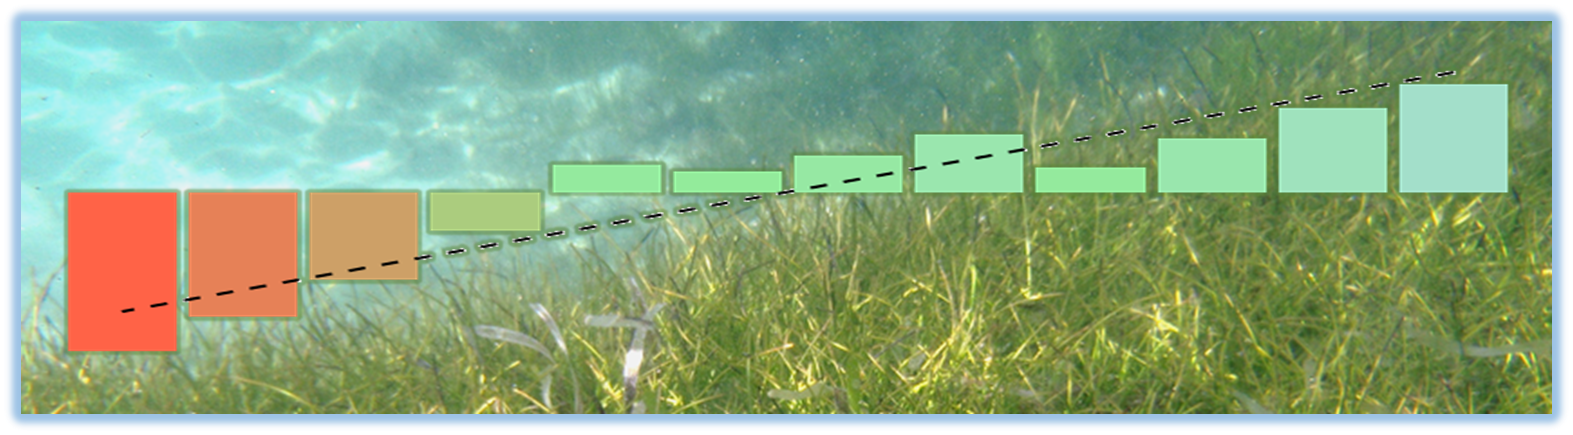
\includegraphics[width=0.7\textwidth]{fig/title_pic.png}}
}

%%%%%%
\begin{frame}
\titlepage
\end{frame}

\section{Background}

%%%%%%
\begin{frame}{Overview}
A mixture of things...\\~\\
\begin{itemize}
\item What is NERSS/SWMP and motivation for creating the package \\~\\
\item The process of package development \\~\\
\item What can SWMPr do \\~\\
\item What has SWMPr done \\~\\
\end{itemize}
\end{frame}

\section{Motivation}

%%%%%%
\begin{frame}{What is NERRS/SWMP?}{}
{\bf NERRS}\\
National Estuarine Research Reserve System, established by Coastal Zone Management Act of 1972.  Address goals for \Bigtxt{long-term research}, \Bigtxt{monitoring}, \Bigtxt{education}, and \Bigtxt{stewardship} for more effective coastal management.\\~\\
{\bf SWMP}\\
System Wide Monitoring Program, initiated in 1995 to provide \Bigtxt{continuous monitoring} data at over 300 stations in in each of the 28 NERRS reserves \\~\\
\end{frame}

%%%%%%
\begin{frame}{What is NERRS/SWMP?}
\centerline{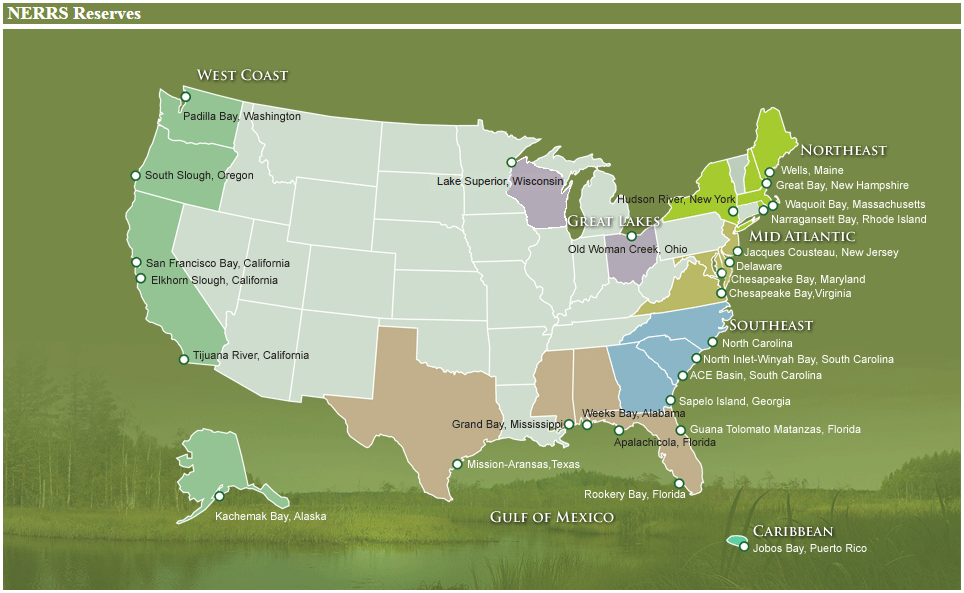
\includegraphics[width = 0.9\textwidth]{fig/NERRS_locations.png}}
\tiny
\flushright
\href{http://nerrs.noaa.gov/ReservesMap.aspx}{http://nerrs.noaa.gov/ReservesMap.aspx}
\end{frame}

%%%%%%
\begin{frame}{What is NERRS/SWMP?}
Each reserve has fixed, continuous monitoring stations for \Bigtxt{water quality} (15 min), \Bigtxt{meteorology} (15 min), and \Bigtxt{nutrients} (monthly)\\~\\
The parameters for a station are specific to the parameter type \\~\\
\begin{columns}[t]
\begin{column}{0.3\textwidth}
\Bigtxt{Water quality} \\~\\
temp, spcond, sal, do\_pct, do\_mgl, depth, cdepth, level, clevel, ph, turb, chlfluor
\end{column}
\begin{column}{0.3\textwidth}
\Bigtxt{Meteorology} \\~\\
atemp, rh, bp, wspd, maxwspd, wdir, sdwdir, totpar, totprcp, cumprcp, totsorad \\~\\
\end{column}
\begin{column}{0.3\textwidth}
\Bigtxt{Nutrients} \\~\\
po4f, chla\_n, no3f, no2f, nh4f, no23f, ke\_n, urea
\end{column}
\end{columns}
\end{frame}

%%%%%%
\begin{frame}[t]{What is NERRS/SWMP?}
Data maintained by the Centralized Data Management Office (\href{http://cdmo.baruch.sc.edu/}{CDMO})\\~\\
\centerline{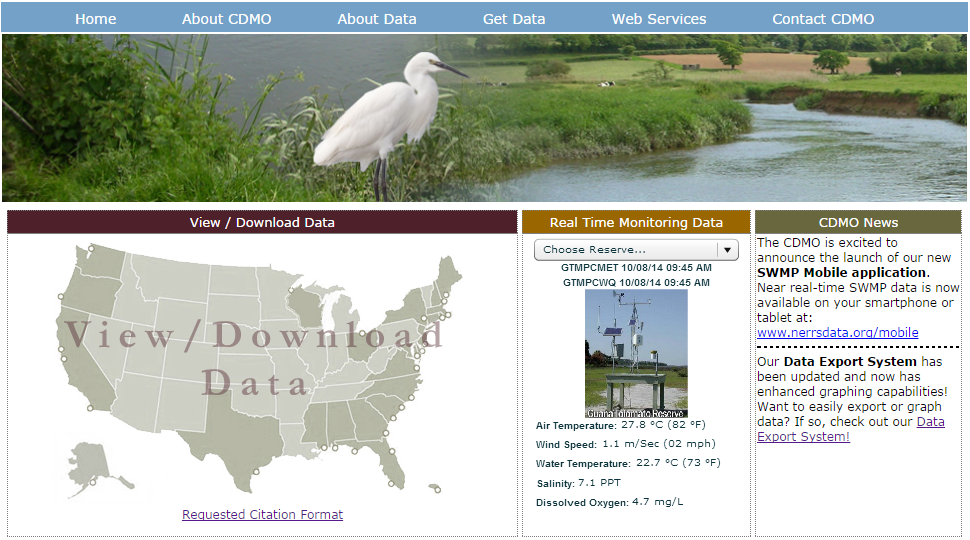
\includegraphics[width = \textwidth]{fig/cdmo_front.png}}
\end{frame}

%%%%%%
\begin{frame}[t]{What is NERRS/SWMP?}
As of April 10, $>$ 58 million SWMP data records available from CDMO\\~\\
Raw data will look like this...\\~\\
\centerline{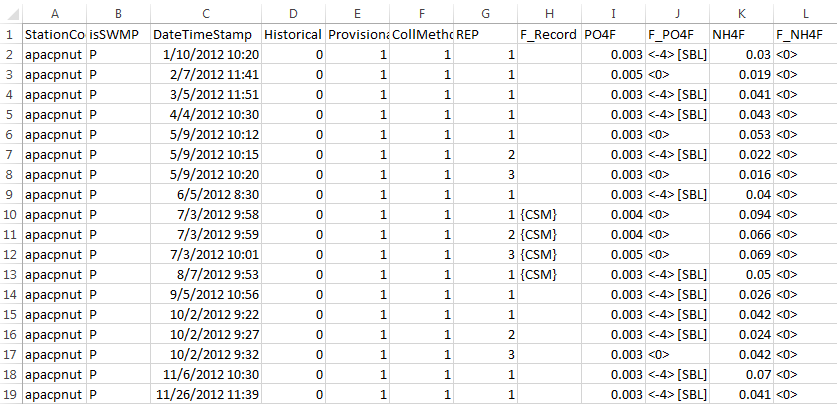
\includegraphics[width = 0.9\textwidth]{fig/qaqc_ex.png}}
\end{frame}

%%%%%%
\begin{frame}{What is the problem?}
An invaluable data source but no recent comparative analyses between systems \\~\\
NERRS researchers, managers, and technicians need more tools for trend analysis \\~\\
Some specific issues:\\~\\
\begin{itemize}
\item Knowing what data to use and how to obtain
\item Dealing with QAQC columns or removing `bad' observations
\item Combining data for comparison
\item Issues inherent with time series, e.g., signal vs. noise, data quantity
\end{itemize}
\end{frame}

%%%%%%
\begin{frame}[fragile]{What is the (potential) solution?}
\centerline{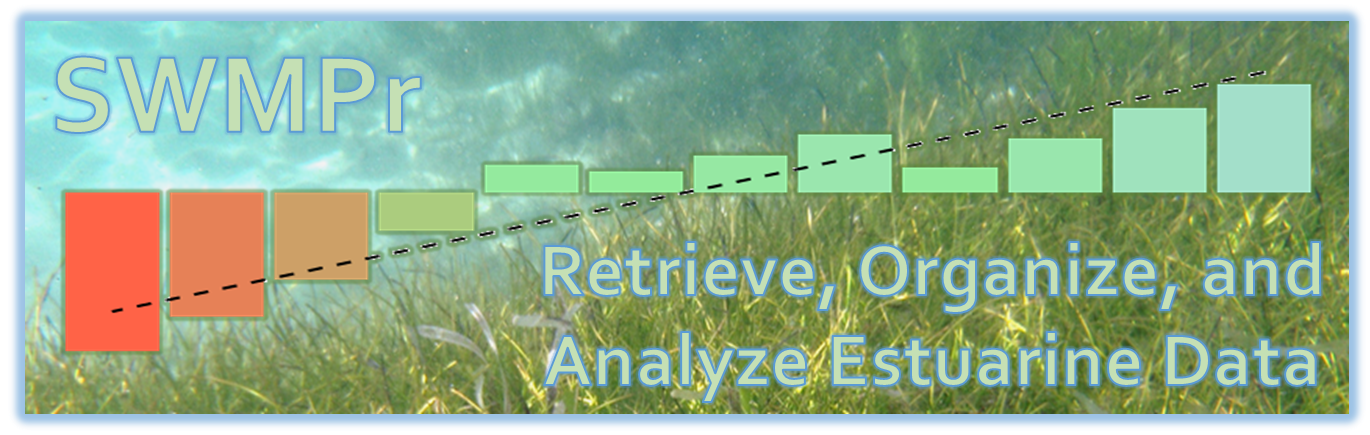
\includegraphics[width = 0.9\textwidth]{fig/swmpr_logo.png}}
\vspace{0.1in}
SWMPr v2.0.0 is now available on \href{http://cran.r-project.org/web/packages/SWMPr/index.html}{CRAN}!
\begin{knitrout}
\definecolor{shadecolor}{rgb}{0.929, 0.973, 0.984}\color{fgcolor}\begin{kframe}
\begin{alltt}
\hlstd{> }\hlkwd{install.packages}\hlstd{(}\hlstr{'SWMPr'}\hlstd{)}
\hlstd{> }\hlkwd{library}\hlstd{(SWMPR)}
\end{alltt}
\end{kframe}
\end{knitrout}
Currently no vignette, but working on a manuscript
\end{frame}

\section{Package development}

%%%%%%
\begin{frame}[fragile]{The process of package development}
The development version lives on GitHub: \href{https://github.com/fawda123/SWMPr}{https://github.com/fawda123/SWMPr} \\~\\
The package development process was much simplified using RStudio and the Hadleyverse (specifically \href{http://cran.r-project.org/web/packages/devtools/index.html}{devtools}, \href{http://cran.r-project.org/web/packages/roxygen2/index.html}{roxygen2}) \\~\\
In RStudio, create a package template: \\~\\
\texttt{File $>$ New Project $>$ New Directory $>$ R Package}, with options for Git version control \\~\\
Package does not have to be on CRAN to distribute...
\end{frame}

%%%%%%
\begin{frame}{The process of package development}
Follow the advice here: \href{http://r-pkgs.had.co.nz/}{http://r-pkgs.had.co.nz/}\\~\\
\centerline{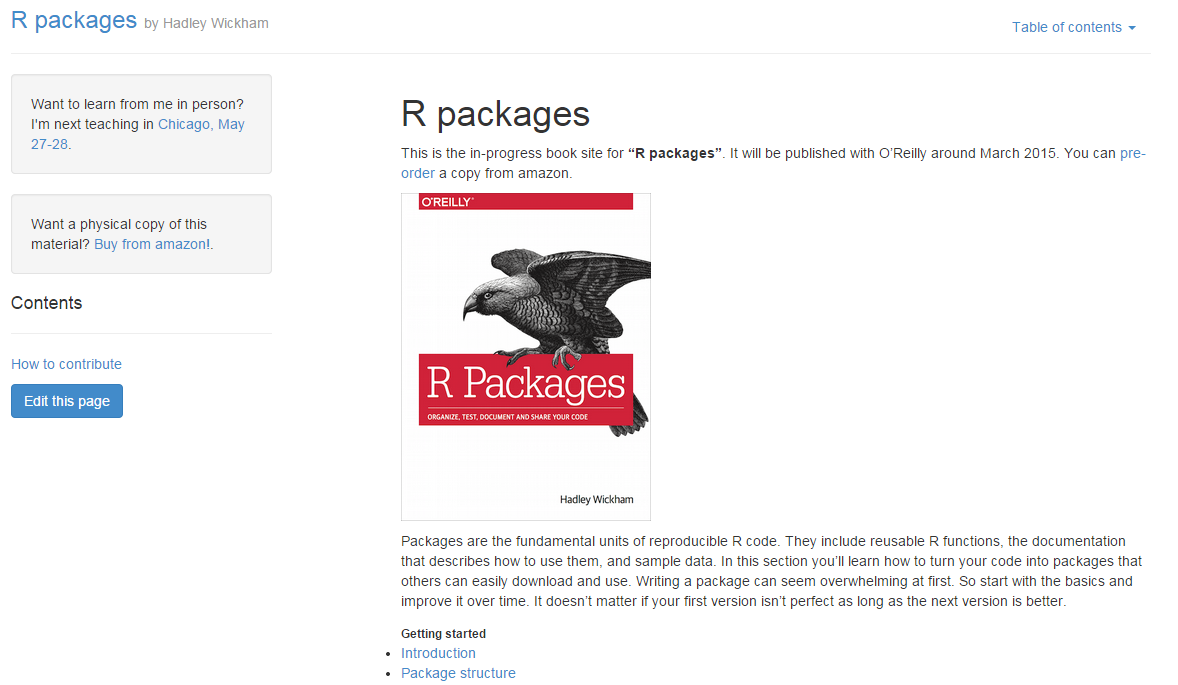
\includegraphics[width = 0.9\textwidth]{fig/hadley_book.png}}
\end{frame}

\section{SWMPr capabilities}

%%%%%%
\begin{frame}[t]{What can SWMPr do?}
SWMPr functions are grouped into three categories that describe their use in the `data workflow' \\~\\
\begin{columns}[t]
\begin{column}{0.3\textwidth}
\Bigtxt{Retrieve}\\~\\
\small{
\texttt{all\_params}\\
\texttt{all\_params_dtrng}\\
\texttt{import\_local}\\
\texttt{import\_remote}\\
\texttt{single\_param}\\
\texttt{site\_codes}\\
\texttt{site\_codes\_ind}
}
\end{column}
\begin{column}{0.3\textwidth}
\Bigtxt{Organize}\\~\\
\small{
\texttt{comb}\\
\texttt{qaqc}\\
\texttt{qaqcchk}\\
\texttt{rem\_reps}\\
\texttt{setstep}\\
\texttt{subset}\\
}
\end{column}
\begin{column}{0.3\textwidth}
\Bigtxt{Analyze}\\~\\
\small{
\texttt{aggreswmp}\\
\texttt{aggremetab}\\
\texttt{ecometab}\\
\texttt{decomp}\\
\texttt{decomp\_cj}\\
\texttt{hist}\\
\texttt{lines}\\
\texttt{na.approx}\\
\texttt{plot}\\
\texttt{plot\_metab}\\
\texttt{plot\_summary}\\
\texttt{smoother}\\
}
\end{column}
\end{columns}
\end{frame}

%%%%%%
\begin{frame}{How are data \Bigtxt{retrieved}?}
The first challenge is to determine the station, parameter, and date range of interest - Check the available data on the CDMO website \\~\\
Also familiarize yourself with the NERRS/SWMP naming convention\\~\\  
\Bigtxt{Site} (reserve), \Bigtxt{station}, and \Bigtxt{parameter type} are identified by a 7 or 8 character name \\~\\
E.g., elkcwmet \\~\\
\begin{itemize}
\item elk: site, Elkhorn Slough
\item cw: station, Caspian Weather Station
\item met: parameter type (weather)
\end{itemize}
\end{frame}

%%%%%%
\begin{frame}[t]{How are data \Bigtxt{retrieved}?}
SWMP data can be imported from CDMO into R three ways\\~\\
1) From a local path: \texttt{import\_local} \\~\\
Advantages: \\~\\
\begin{itemize}
\item Ideal for large datasets
\item Most recent data \\~\\
\end{itemize}
Disadvantages: \\~\\
\begin{itemize}
\item Outside of R
\item Only works for one type of data request from CDMO
\end{itemize}
\end{frame}

%%%%%%
\begin{frame}[t]{How are data \Bigtxt{retrieved}?}
SWMP data can be imported from CDMO into R three ways\\~\\
2) retrieve SWMP data from a third-party server: \texttt{import\_remote}, \\~\\
Advantages:\\~\\
\begin{itemize}
\item Fast import!
\item No requests to CDMO\\~\\
\end{itemize}
Disadvantages:\\~\\
\begin{itemize}
\item Data are not current
\item Requires further processing - date subsets, etc.
\end{itemize}
\end{frame}

%%%%%%
\begin{frame}[t]{How are data \Bigtxt{retrieved}?}
SWMP data can be imported from CDMO into R three ways\\~\\
3) Use the existing CDMO web services to import directly:  \texttt{single\_param}, \texttt{all\_params}, \texttt{all\_params\_dtrng} \\~\\
Advantages: \\~\\
\begin{itemize}
\item Current
\item Customized requests\\~\\
\end{itemize}
Disadvantages:\\~\\
\begin{itemize}
\item IP address must be registered
\item Quantity severely limited
\end{itemize}
\end{frame}

%%%%%%
\begin{frame}[fragile,t]{How are data \Bigtxt{retrieved}?}
The best approach depends on your needs \\~\\
The end result is the same - data are imported as a \texttt{swmpr} S3 object
\begin{knitrout}
\definecolor{shadecolor}{rgb}{0.929, 0.973, 0.984}\color{fgcolor}\begin{kframe}
\begin{alltt}
\hlstd{> }\hlstd{dat} \hlkwb{<-} \hlkwd{import_remote}\hlstd{(}\hlstr{'kacsswq'}\hlstd{)}
\hlstd{> }\hlkwd{class}\hlstd{(dat)}
\end{alltt}
\begin{verbatim}
## [1] "swmpr"      "data.frame"
\end{verbatim}
\begin{alltt}
\hlstd{> }\hlkwd{names}\hlstd{(}\hlkwd{attributes}\hlstd{(dat))}
\end{alltt}
\begin{verbatim}
## [1] "names"       "row.names"   "class"       "station"    
## [5] "parameters"  "qaqc_cols"   "date_rng"    "timezone"   
## [9] "stamp_class"
\end{verbatim}
\end{kframe}
\end{knitrout}
\end{frame}

%%%%%%
\begin{frame}[fragile,t]{How are data \Bigtxt{retrieved}?}
The remaining functions have \texttt{swmpr} methods
\begin{knitrout}\small
\definecolor{shadecolor}{rgb}{0.929, 0.973, 0.984}\color{fgcolor}\begin{kframe}
\begin{alltt}
\hlstd{> }\hlkwd{methods}\hlstd{(}\hlkwc{class} \hlstd{=} \hlstr{'swmpr'}\hlstd{)}
\end{alltt}
\begin{verbatim}
##  [1] aggremetab.swmpr*   aggreswmp.swmpr*   
##  [3] comb.swmpr*         decomp.swmpr*      
##  [5] decomp_cj.swmpr*    ecometab.swmpr*    
##  [7] hist.swmpr*         lines.swmpr*       
##  [9] na.approx.swmpr*    plot.swmpr*        
## [11] plot_metab.swmpr*   plot_summary.swmpr*
## [13] qaqc.swmpr*         qaqcchk.swmpr*     
## [15] rem_reps.swmpr*     setstep.swmpr*     
## [17] smoother.swmpr*     subset.swmpr*      
## 
##    Non-visible functions are asterisked
\end{verbatim}
\end{kframe}
\end{knitrout}
\texttt{swmpr} objects also inherit methods from the \texttt{data.frame} class
\end{frame}

%%%%%%
\begin{frame}[fragile,t]{How are data \Bigtxt{organized}?}
Data organization depends on the analysis needs - it is neither fun nor straightforward (common opinion, not mine) \\~\\
What are some challenges?\\~\\
\begin{itemize}
\item Imported data have QAQC columns
\item Extra columns/rows
\item Maybe we don't care about all the parameters
\item Data from separate sites are in separate objects \\~\\
\end{itemize}
The \Bigtxt{organize} functions are specific to the SWMP data but many of the principles apply to generic time series
\end{frame}

%%%%%%
\begin{frame}[fragile]{How are data \Bigtxt{organized}?}
A relevant example - we want to compare time series from different sites\\~\\
\begin{itemize}
\item Data may have arbitrary time steps that do not match between sites \\~\\
\item Date ranges may also differ \\~\\
\end{itemize}
The \texttt{setstep} and \texttt{comb} functions address these issues! \\~\\
\begin{knitrout}
\definecolor{shadecolor}{rgb}{0.929, 0.973, 0.984}\color{fgcolor}\begin{kframe}
\begin{alltt}
\hlstd{> }\hlstd{met} \hlkwb{<-} \hlkwd{import_remote}\hlstd{(}\hlstr{'apaebmet'}\hlstd{)}
\hlstd{> }\hlstd{wq} \hlkwb{<-} \hlkwd{import_remote}\hlstd{(}\hlstr{'apacpwq'}\hlstd{)}
\hlstd{> }\hlstd{dat} \hlkwb{<-} \hlkwd{comb}\hlstd{(met, wq)} \hlcom{# tada!}
\end{alltt}
\end{kframe}
\end{knitrout}
\end{frame}

%%%%%%
\begin{frame}{How are data \Bigtxt{organized}?}
The \texttt{setstep} function is used within \texttt{comb} to standardize the time steps for each input object \\~\\
A tricky problem - actual observations which may occur on an arbitrary step must be matched to a set time step\\~\\
This function uses `fast-ordered joins' from the \href{http://cran.r-project.org/web/packages/data.table/index.html}{data.table} package using the `nearest' method\\~\\
Also must define a threshold for matching: +/- some buffer of allowance beyond which matches are discarded \\~\\
\end{frame}

%%%%%%
\begin{frame}{How are data \Bigtxt{organized}?}
Mechanistically, \texttt{setstep} does the following for each data object: \\~\\
\begin{itemize}
\item Create a continuous `master' time series at defined step using first/last time stamps
\item Match existing observations to standardized using `nearest' join method
\item Calculate difference in time between matched and standardized step, discard those beyond threshold \\~\\
\end{itemize}
Standardized datasets are then combined by absolute matching of time steps
\end{frame}

%%%%%%
\begin{frame}[fragile]{How are data \Bigtxt{organized}?}
\begin{knitrout}\small
\definecolor{shadecolor}{rgb}{0.929, 0.973, 0.984}\color{fgcolor}\begin{kframe}
\begin{alltt}
\hlstd{> }\hlkwd{dim}\hlstd{(met)}
\end{alltt}
\begin{verbatim}
## [1] 490847     11
\end{verbatim}
\begin{alltt}
\hlstd{> }\hlkwd{dim}\hlstd{(wq)}
\end{alltt}
\begin{verbatim}
## [1] 455808     13
\end{verbatim}
\begin{alltt}
\hlstd{> }\hlcom{# standardize time step to two hours}
\hlstd{> }\hlcom{# maximum difference for matching 30 minutes}
\hlstd{> }\hlcom{# combine only overlapping time ranges}
\hlstd{> }\hlstd{dat} \hlkwb{<-} \hlkwd{comb}\hlstd{(wq, met,} \hlkwc{timestep} \hlstd{=} \hlnum{120}\hlstd{,} \hlkwc{differ} \hlstd{=} \hlnum{30}\hlstd{,}
\hlstd{+ }  \hlkwc{method} \hlstd{=} \hlstr{'intersect'}\hlstd{)}
\hlstd{> }\hlkwd{dim}\hlstd{(dat)}
\end{alltt}
\begin{verbatim}
## [1] 56977    23
\end{verbatim}
\end{kframe}
\end{knitrout}
\end{frame}

%%%%%%
\begin{frame}[fragile]{How are data \Bigtxt{organized}?}
\begin{knitrout}\small
\definecolor{shadecolor}{rgb}{0.929, 0.973, 0.984}\color{fgcolor}\begin{kframe}
\begin{alltt}
\hlstd{> }\hlkwd{head}\hlstd{(dat,} \hlnum{4}\hlstd{)}
\end{alltt}
\begin{verbatim}
##         datetimestamp atemp rh   bp wspd maxwspd wdir
## 1 2001-12-31 23:00:00     4 69 1017    4      NA  347
## 2 2002-01-01 01:00:00     3 75 1017    3      NA    9
## 3 2002-01-01 03:00:00     2 77 1018    3      NA  331
## 4 2002-01-01 05:00:00     1 82 1019    4      NA    0
##   sdwdir totpar totprcp totsorad temp spcond sal do_pct
## 1     NA      0      NA       NA   NA     NA  NA     NA
## 2     NA      0      NA       NA   12     37  24    104
## 3     NA      0      NA       NA   12     40  26     99
## 4     NA      0      NA       NA   11     42  26     98
##   do_mgl depth cdepth level clevel ph turb chlfluor
## 1     NA    NA     NA    NA     NA NA   NA       NA
## 2     10     2     NA    NA     NA NA    3       NA
## 3      9     2     NA    NA     NA NA    4       NA
## 4      9     2     NA    NA     NA NA    5       NA
\end{verbatim}
\end{kframe}
\end{knitrout}
\end{frame}

%%%%%
\begin{frame}{How are data \Bigtxt{analyzed}?}
Time series analysis can be very general or very specific...\\~\\

\end{frame}

\section{SWMPr applications}

%%%%%
\begin{frame}{Applications}

\end{frame}

\end{document}

